\chapter{Design}
-objectives
-use cases (actors)
-architecture of backend
-design patterns
-gui (with screenshots)
\section{Objectives}
\par \textbf{Visability} -  It should be visible to the user what are the functions that are available. This includes being able to distinguish actions from informative text. This can be ensured through the use of buttons that are highlighted. This would allow to provide an application that can be picked up and used with minimal to none training. Therefore, it would be beneficial to the growth of the systems use, by attracting more users through its simplicity of use. This can be completed by providing a simple and intuitive User Interface (UI), where buttons are highlighted, and the interface is not cluttered with actions, instead just providing what is necessary. The timeline produced will be available in three different formats: graphically in the system, as a PDF file, or as a JSON. The latter is the only one that is not a graphical representation, while the other two do.
\par \textbf{Efficient} - The time spent to perform tasks should be reasonable in the context of the input. This can be further expressed in mathematical notation of Big-Oh. If an algorithm takes an input of size $n$, and roughly performs $n$ operations to produce a result, then the algorithm is said to have a runtime of Big-Oh of $n$. This allows the efficiency of an algorithm to be compared to other algorithms, and for the run-time to be scaled to larger inputs. An objective would be to avoid having a run-time, a Big-Oh, that is exponential. Since for a small $n$ the run-time is large, therefore, for a large $n$ it is infeasible for a result to be produced in time. This objective can be completed through the use of Threads. A Thread is a lightweight processor computation unit. Using more than one-thread allows for tasks to be carried out in parallel. Therefore, if the input is $n$ documents, and there are $n$ threads, then the running time of the system would be the greatest running time of all the documents being carried out. Since if all documents are being processed in parallel, and completely independently of each other, the one document that takes the longest to be processed will give the time of processing all of the documents (cite). The amount of threads running in parallel should be an editable setting to the user, as they may wish to reduce the load of running many threads in parallel in the case they are doing other work on their machine, or they may wish to use the maximum amount of possible threads they can.
\par \textbf{Effective} - The system should meeet its purpose. That is, its task is to take as input documents and produce a timeline. Thereby, the system should provide the user options to load documents, and then provide a graphical response. In the case where no response can be produced, i.e. due to the document encoding not being parsable, then the system should not attempt indefinetely to produce a timeline with that document, and instead produce an empty timeline. 
\section{Use Cases}
\par A use case is a task a actor in the system may want to perform. An actor is any type of user of the system. In this case, the user can be a law professional that requires to have a general understanding of a given set law-realted documents. Therefore, it can be assumed that the user does not necessarily have experience with NLP, and the tasks that are involved in processing the document. It should be transparent to the user how the documents are being parsed, and only if they are interested would they require to look at the available source-code. The technical skill of the user does not need to be of an expert, as the tasks required are to provide documents, and then from the resulting timeline they can traverse it and perform their analysis. In some cases, the user may produce their own graphical representation of a timeline and just use the produced JSON of the system.
\par The use cases of the system are given by the requirements, and they are found below. //use case stick figure diagram
\begin{enumerate}
  \item Load Documents
  \begin{enumerate}
    \item Primary Actor: User
    \item Goal: load set of given documents, where the document file types can be  .pdf, .docx, or .txt.
    \item Main Sequence:
	\begin{enumerate}
		\item User selects the "Load Documents" option.
		\item System prompts a File Selector.
		\item User selects set of documents and the base dates (or reference dates) to use with them.
		\item System responds with timeline of events.
	\end{enumerate}
  \end{enumerate}
  \item Swap from Timeline to Document
   \begin{enumerate}
	\item Primary Actor: User
	\item Goal: show the sentence, in context, that produced the given event.
	\item Main Sequence:
	\begin{enumerate}
		\item User selects event.
		\item System responds with dialog to "Edit Event" or "Go to Document".
		\item User selects "Go to Document" option.
		\item System opens new window with the text of the document where the event originates from, with the sentence that produced it highglighted.
	\end{enumerate}
    \end{enumerate}
   \item Edit Event
      \begin{enumerate}
	\item Primary Actor: User
	\item Goal: modify the data of an event.
	\item Main Sequence:
	\begin{enumerate}
		\item User selects event.
		\item System responds with dialog to "Edit Event" or "Go to Document".
		\item User selects "Edit Event" option.
		\item System responds with dialog with the data of the event set in fields.
		\item User edits the data as needed.
		\item System validates the entered data, and saves.
	\end{enumerate}
     \end{enumerate}
   \item Save Timeline
    \begin{enumerate}
	\item Primary Actor: User
	\item Goal: save the produced timeline as a PDF or JSON.
	\item Main Sequence:
	\begin{enumerate}
		\item User selects "Save To..." option.
		\item System responds with option dialog to select the file format to save.
		\item User selects the needed file format.
		\item System responds with File Selector.
		\item User selects the location to save the timeline.
		\item System generates the required data to save the timeline in the desired format and attempts to save it in the system.
	\end{enumerate}
    \end{enumerate}
\end{enumerate}
//note load documents use case includes adding to an existing timeline, user is the person using the system, edit event incl delete, checks for invalid data, file not available
\par The main sequence are the steps of the interaction in the use case to reach the desired goal. An error can occur during the interaction. It should be the systems responsibility to deal with the error, and not end the execution of the program. The primary actor, is the agent, or entity that initiates the use case (cite or footnote).
\par It should be noted that loading a document includes both when it is the first set of documents to be loaded, i.e. the timeline is empty, and when there is already a populated timeline. In the latter case, it would be beneficial to discard duplicated events. A duplicated event is one where it is produced from the same file, using the same reference date, and the data is equal. This is done to not clutter the timeline with events that are repeated, as the timeline should be efficient in the data it provides, i.e. describe the events in the document with as little as possible of additional data. It can occur that two documents produce the same event, these should not count as duplicated, as the event may have a different context depending on what file it is from. The reference date is included, as for the same document different events may be produced depending on the reference date used for that document. 
\par When an event is being edited, the user should have the option to delete said event. It can be that the system produced an event that is not relevant for the user, or another event describes it. This can be the case when a set of closely related documents are loaded, and two or more events have the same meaning, but are not direct duplicates as they originate from separate files. In addition, when the user edits the data of an event, validation checks are performed before the changes are saved. It can occur that the modification inserted invalid data. For example, if the date of an event is modified but instead of a new date being set, text is placed. In the case of the event occuring during a range of dates, i.e. it has a start date and end date, a plausible validation check should be that the second date does not occur before the first. The system can do these checks before it attempts to save the modifications, and in cases where the validations fails, the changes should not be saved, instead the user should be prompted to enter correct data or cancel the action. The system should inform the user of where they validation failed, to allow them to correct the data.
\par It can occur that the desired location of where the timeline should be saved is unavailable. This can be due to the system not having write access to that part of the Operating System, or the file which is being overwritten is in use (i.e. another process locked the file (cite or footnote)).
\section{Architecture}
\par The architecture of a system, is the structure of the components of the system\footnote{\url{https://msdn.microsoft.com/en-gb/library/ee658098.aspx}}. It focuses on the back-end, or logic, of the system as opposed to the graphical, or front-end task. A good software architecture is one where the components of the system are encapsulated with other related components. For this project, the software architecture has been produced using Unified-Modelling Language (UML). In UML, components or classes are represented by a rectangle, with their available functions listed. The architecture of the whole system is presented in the figure below (Figure \ref{fig:fullArch}). We will look at each package individually.
\begin{figure}[H]
\caption{Full UML Architecture of Automated Timeline Extraction system.}
\label{fig:fullArch}
\includegraphics[width=\linewidth]{fullarch.png}
\centering
\end{figure}
\subsection{Process Package}
\par The core of the system is the process package (see Figure \ref{fig:process}). The architecture used here, is that interaction is done through ProcessFiles. A list of files is passed in, along with their data (such as the file name, its path, or the creation date used). Each file is processed in parallel. The maximum number of parallel processing that can be done is given by the settings of the system (in the settings package). This is the maximum number of threads that can be ran at any given point. However, in the implemented system one more thread should be added to the count, as the graphical user interface always runs on a separate thread. The idea is that if the maximum setting is $n$, then at any given point at most $n$ files are being processed. Whenever one file finishes processing, another begins to be processed. As mentioned before, if $n$ files are allowed to process at any given point, and the input size of documents is $n$, then the time it takes for the system to process all the documents is given by the greates maximum time to process one of the $n$ files. The pseudo-code for this is given below (see Algorithm \ref{alg:processFiles}), in an actual implementation semaphores can be used. A semaphore is a control data structure to limit how many processes can run in parallel. It is done by acquiring a lock when a process needs to be ran, if a lock is available then the process can run, if no lock is available then the process waits until one is available.
\begin{figure}[h]
\caption{UML of the Processing Package}
\label{fig:process}
\includegraphics[width=\linewidth]{process.png}
\centering
\end{figure}
\begin{algorithm}
\SetKwInOut{Input}{Input}
\SetKwInOut{Output}{Output}
\Input{A list of Files to Process}
\Output{A list of Results}
\ForEach{File in the input list}{
	wait until can run\; \COMMENT if the maximum number of threads running in parallel has not been reached then stop waiting, else wait
	process the file\;
	add the produced Result to the list of Results to return\;
}
return list of Results\;
\caption{Algorithm for processing a list of Files}
\label{alg:processFiles}
\end{algorithm}
\par A Result is the event of a timeline in this system. It holds the start and end date of an event, its subjects, and its summary. The start and end date are determined through the TimelineDate component.
\par When a temporal expression is detected in a sentence, it must be processed to an exact date to be useful. This is done through TimelineDate. It attempts to parse them. In this system, the decision was made to use the StanfordCoreNLP suite \footnote{\url{http://stanfordnlp.github.io/CoreNLP/}}. It is a well-known and tested tool for Natural Language Processing. Other tools exist, such as ApacheNLP, however Stanford's tool has a larger set of documentation and support, as well as being a thread-safe and efficient tool. Thread-safe refers to the ability to share this tool between separate processes without having to worrry about concurrency issues. 
\par When a file is processed, its text is extracted, and this is then passed through the Engine. The Engine is responsible for producing the Results for that file. It identifies sentences with dates, and for those it extracts subjects such as people, locations, money, etc. In addition, it implements the Hedge-Trimmer discussed in the Background Chapter.
\subsection{System Package}
//talk about system to be shared throughout the system (same data shared)
\par The system package holds the system and settings components (see Figure \ref{fig:system}). It is responsible for providing global settings, such as the maximum number of threads to be ran in parallel, the threshold value used in the sumamry algorithm, and graphical settings such as the width and height of the window. An interesting aspect of this package is the SystemState. As the system moves from start, to processing files and then finishing the processing. This can be modelled in the system. When files are passed through the process package, the state of the system is changed. This allows for the graphical representation of the system to be decoupled of the logic, as it can use the system state to determine when certain actions are available, when a loading bar needs to be shown, and when a timeline should be displayed. This component is shared throughout the system, as it contains data that is required in other components, both for the logical aspects of the system and the graphical aspects.
\begin{figure}[H]
\caption{UML of the System Package}
\label{fig:system}
\includegraphics[width=\linewidth]{system.png}
\centering
\end{figure}
\subsection{Ranges Package}
//trees of ranges with results, algorithm, example, running time
\par The ranges package was one of the later packages developed (see Figure \ref{fig:ranges}). Its focus is on placing already produced Results into ranges of dates (see the Algorithm \ref{alg:produceRanges}). A Range is defined by a start and end date. A Result is placed within this Range if it has the exact same start and end date, if this is not the case then it attempts to look at the children of that Range. If it is not possible to place the Result in a Rangeor its children then another root Range is checked. If after checking all Ranges this is still not possible, then a new separate root Range is created using the Results dates and the Result is placed there.This allows to order events within each other, such that if one event occurred during the period of a longer event, than that event will be contained by the other. 
\begin{figure}[H]
\caption{UML of the Ranges Package}
\label{fig:ranges}
\includegraphics[width=\linewidth]{ranges.png}
\centering
\end{figure}
\begin{algorithm}
\SetKwInOut{Input}{Input}
\SetKwInOut{Output}{Output}
\Input{A list of Results}
\Output{A list of Range roots, i.e. a forest of Ranges}
sort the list of Results by the number of days in between the start and end date in descending order\;
\ForEach{Result in the sorted list}{
	attempt to add it to one of the existing Range roots\;
	\If{failed to add to existing Range}{
		make a new Range using the data of the Result\;
		add the new Range to the list of Range roots\;
	}
}
return list of Range roots\;
\caption{Algorithm for placing Results in Ranges}
\label{alg:produceRanges}
\end{algorithm}
\par The Results are sorted by the range of the start and end date, i.e. the numer of days between the two. A Result that only has one date, because it just occurred on that specific date, has a range of 0. The Results with the largest ranges are added first as it is more likely that in the possible dates inbetween their start and end date, there will be Results that have start and end dates there. This leads to the production of a tree, which will be shown below. Where the root is a Range with a start and end date that encapsulates all the start and end dates that are in the tree. In some cases it will be necessary to expand the dates of a Range if it is the case that a Result has an event that overlaps with the dates of the Range. This will then lead to have a Range that has no results, but has two children, the newly made Range for the Result that is being added, and a subtree which was Range that was being overlapped.
\par For example, if you have the two Results presented in the table \ref{fig:resultsTable} and the pre-existing tree in Figure \ref{fig:rangeTreePre}. The Results would be sorted by their range, such that the second result would be the first to be added. This would produce the tree in Figure \ref{fig:rangeTree1}. Aftwerwards, the first Result in the table would be added, producing the tree in Figure \ref{fig:rangeTree2}. In the Figure \ref{fig:rangeTree2}, the following occurred: it was determined that the Result that was being added overlapped an existing Range, so a new Range was formed that would encapsulate the previous Range and the new Result by extending the start and end dates appropriately. Then a new Range was made that held the Result to be added data, and along with the old Range it was added to the children of the new expanded Range.
\par As can be seen from the last tree produced, the largest start-end date pair encapsulates the smaller start-end date pair, and this is done recursively. This allows for when a list of Results needs to be produced, for example for a Timeline, and the aim is to show which Results happened around the same time period, as Results that overlap with dates are encapsulated.
\begin{figure}[h]
\begin{center}
\begin{tabular}{ |c|c|c| } 
 \hline
Result & Start Date & End Date \\
\hline
\hline
1 & 12-12-2016 & 18-12-2016 \\
2 & 13-12-2016 & 20-12-2016 \\
 \hline
\end{tabular}
\end{center}
\caption{Example Results Start and End Date}
\label{fig:resultsTable}
\end{figure}
\begin{figure}[h]
\resizebox{\linewidth}{!}{
\Tree
 [.{01-01-1980  $\shortrightarrow$ 31-12-2016}
	[.{01-01-2008  $\shortrightarrow$ 31-05-2016} {01-01-2015} ]
	[{01-11-2016} ] 
]
}
\caption{Pre-existing Range Tree}
\label{fig:rangeTreePre}
\end{figure}
\begin{figure}[h]
\resizebox{\linewidth}{!}{
\Tree
 [.{01-01-1980 $\shortrightarrow$ 31-12-2016}
	[.{01-01-2008  $\shortrightarrow$ 31-05-2016} {01-01-2015} ]
	[{13-12-2016  $\shortrightarrow$ 20-12-2016} ]
	[{01-11-2016} ] 
]
}
\caption{Resulting Range Tree after adding the Result: 13-12-2016  $\shortrightarrow$ 20-12-2016}
\label{fig:rangeTree1}
\end{figure}
\begin{figure}
\resizebox{\linewidth}{!}{
\Tree
 [.{01-01-1980 $\shortrightarrow$ 31-12-2016}
	[.{01-01-2008  $\shortrightarrow$ 31-05-2016} {01-01-2015} ]
	[.{12-12-2016  $\shortrightarrow$ 20-12-2016} 
		[{12-12-2016  $\shortrightarrow$ 18-12-2016} ]
		[{13-12-2016  $\shortrightarrow$ 20-12-2016} ]
	]
	[{01-11-2016} ] 
]
}
\caption{Resulting Range Tree after adding the Result: 12-12-2016 $\shortrightarrow$ 18-12-2016}
\label{fig:rangeTree2}
\end{figure}
\subsection{Helpers Package}
\par The helper package holds utility components used throughout the system (see Figure \ref{fig:helpers}). It provides sorting of lists, and the production of JSON and .PDF files for given list of Results. It is a package used in the refactoring of the logic of the system. Refactoring is done to remove repeated components and operations. Thereby having them in one place only instead of being duplicated around the system. The main advantage is that when a change needs to be made, it is made in one place, but if the operations are duplicated throughout the system then that change needs to be carried out at each place. The common functionality that has been placed in one component to use throughout the system includes sorting Results by their dates or by the number of days between the start and end dates.
\begin{figure}[H]
\caption{UML of the Helpers Package}
\label{fig:helpers}
\includegraphics[scale=0.75]{helpers.png}
\centering
\end{figure}
\section{Design Patterns}
\par Design Patters are general solutions to common problems in software development\footnote{\url{https://sourcemaking.com/design_patterns}}. The solutions usually include a system architecture to follow. For this project, the main design patterns are Singleton and Observer.
\par \textbf{Singleton} - This design pattern ensures that only a certain number of instances of a component are available\footnote{\url{http://www.journaldev.com/1377/java-singleton-design-pattern-best-practices-examples}}. In most cases the number of components is restricted to one. The advantage of this pattern is that it allows for global data used throughout the system to be available in one area. As in the System component the NLP processing tool is held, along with the system state, which is used throughout the system at different places, it is beneficial to have this component follow the Singleton pattern. 
\par \textbf{Observer} - This design pattern allows an observee to notify a list of its observers. The observee can be a model, and the the observers its view. This is used to separate the logic of the system from its user interface. It allows for the back-end of the system to be developed completely independently from the front-end. In this system, the front-end will be notified by the back-end. This is then stregnthened further through the different system states available. As the back-end begins processing documents, its state is changed, the front-end can then use this to modify its view appropriately, by retrieving the relevant data and showing the relevant options for that state. If the system were to be developed further, with other graphical interfaces used or added to the pre-existing UI, it can be added in without any issues. Since the logic of the system is independent of its view.
\par \textbf{Model-View Controller} - It is mentioned as a main design pattern of the system, because it is similar to the Observer design pattern. In that it separates the view of data (a model) through a controller. The controller manipulates the data, and applies the appropriate changes in the view. It separates the logicof the system with its view, like an Observer pattern. This design pattern is enforced by many Graphical User Interface (GUI) frameworks, incluiding the one used in this project.
\par Other design patterns are available, however these are the most relevant ones to this project. While the solution for the multi-threading is not a design pattern, it is worth mentioning that precautions have to be taken to independently process each document, which includes the previously mentioned semaphores. 
//singleton, model-view-controller, describe, explain why, and what other options were available
\section{UI}
\par The system is intended to be used by law professionals. However, it can be used by anyone that requires its services of producing timelines, as it will be open-source.  These considerations are taken into account during the development of the User-Interface. For example, as the main data representation of the system is the timeline of events, it is clear that it should occupy a majority of the screen. Options that are not relevant to the current state of the system should be unavailable, while options that are most likely to be used should be highlighted. This aims to achieve the visibility objective of the project.
\par As the main actor can have any level of computer experience, it is important that they are not overloaded with options, and instead are just presented what was is needed. For example, when the system is initially launched, no timeline can be presented as no documents are available to be processed. Thereby, in the Figure presented below (see Figure \ref{fig:startup}) of the launch wireframe, the user is invited to begin using the system by loading documents. It should be noted that a wireframe is a mostly colourless screenshot of what the system should look like.
\begin{figure}[h]
\caption{Wireframe of System at Startup}
\label{fig:startup}
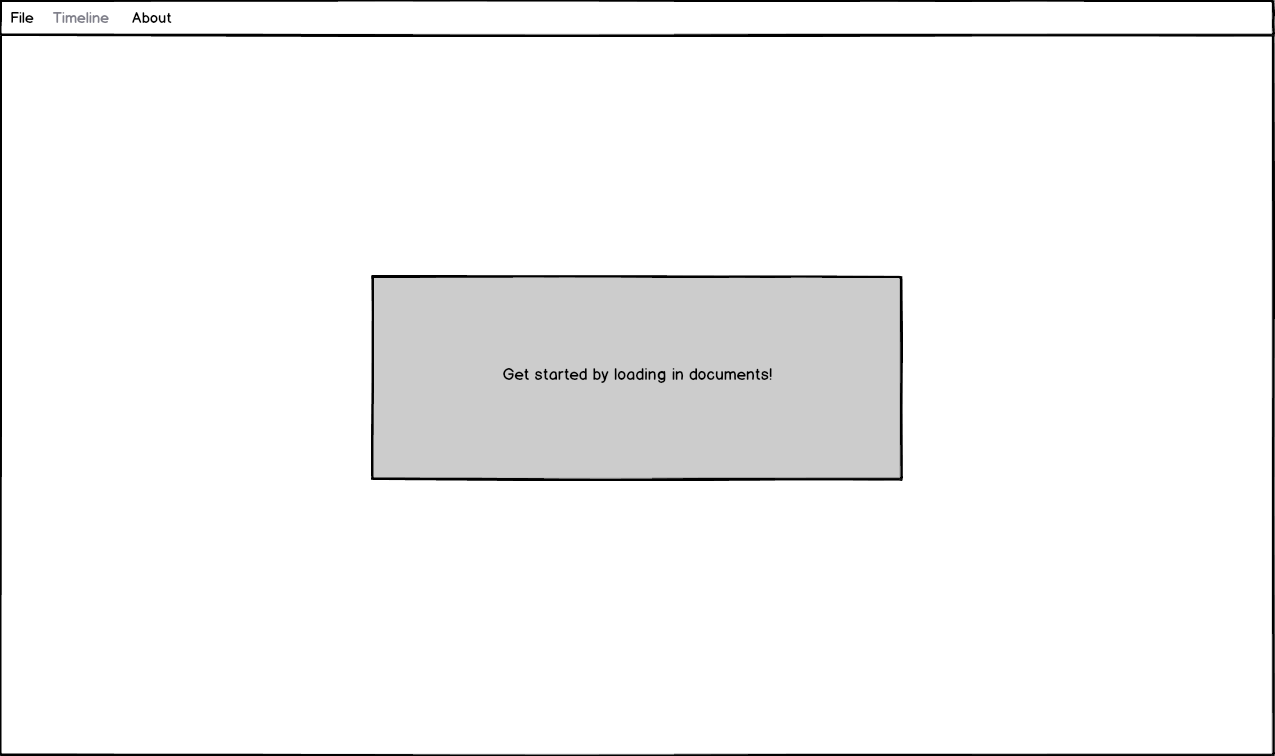
\includegraphics[width=\linewidth]{startup.png}
\centering
\end{figure}
\par From this screen the user can load documents and select the reference dates used for these documents. During this period, the back-end of the system can load any resources it requires to process documents. Once the documents have been chosen by the user, they are presented with a loading dialog, to inform them that the system is processing. After this the timeline should be presented (see Figure \ref{fig:timeline}).
\begin{figure}[h]
\caption{Timeline of System}
\label{fig:timeline}
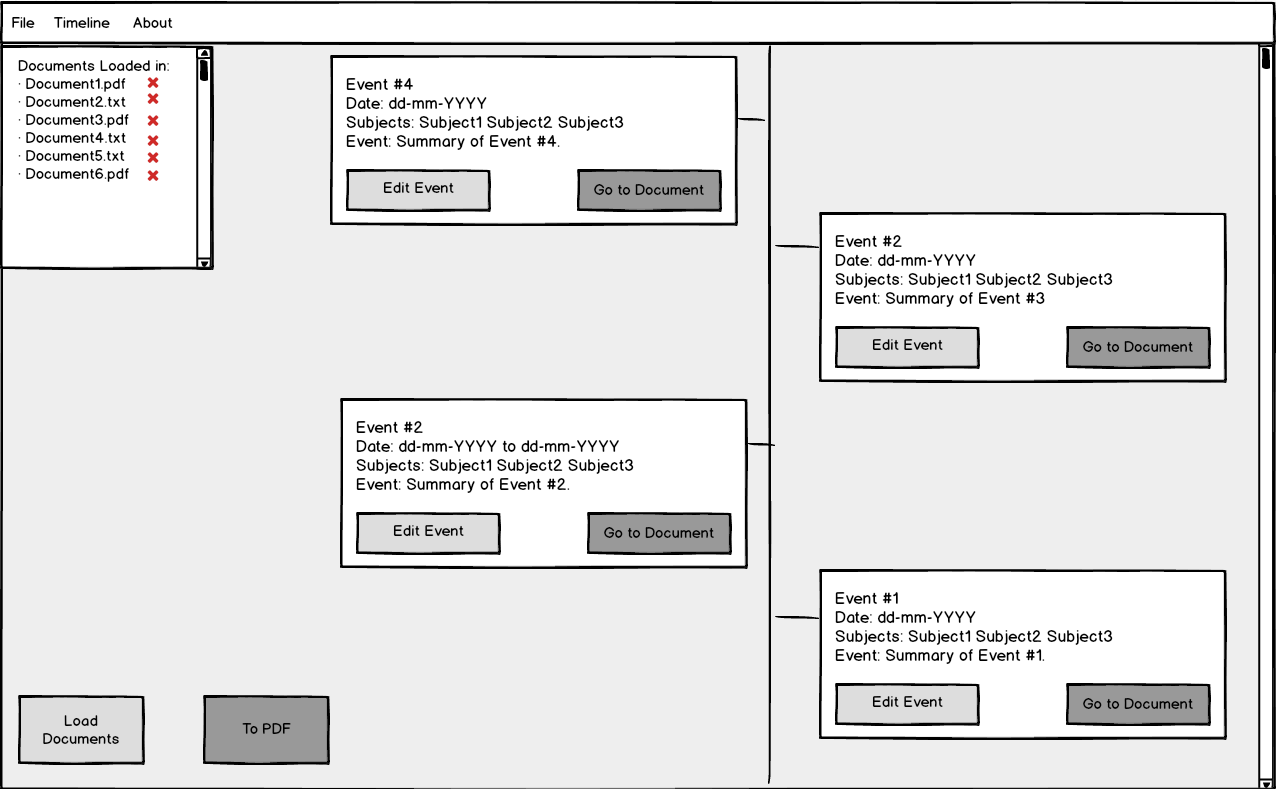
\includegraphics[width=\linewidth]{timeline.png}
\centering
\end{figure}
\par For each event produced by the system, a timeline row will be produced. With each event an option to edit its data is available, which will provide a dialog (see Figure \ref{fig:editDialog}) that includes the option to delete an event, and the option to view the document that produced the given event (see Figure \ref{fig:viewDoc}). In addition, the user is provided valuable information such as which documents have been loaded (with the option to remove them and add to them), and the ability to save the timeline. It should be noted, that as can be seen from Figure \ref{fig:startup} the Timeline option is unvailable as the there is no timeline for the user to interact, while in the Figure \ref{fig:timeline} the option is enabled.
\begin{figure}[h]
\caption{Edit Event Dialog of System}
\label{fig:editDialog}
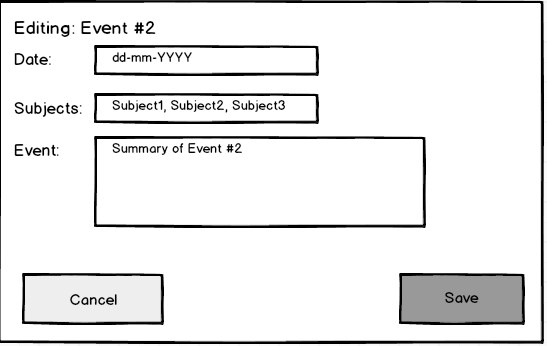
\includegraphics[scale=0.6]{editDialog.png}
\centering
\end{figure}
\begin{figure}[h]
\caption{Document Viewer of System}
\label{fig:viewDoc}
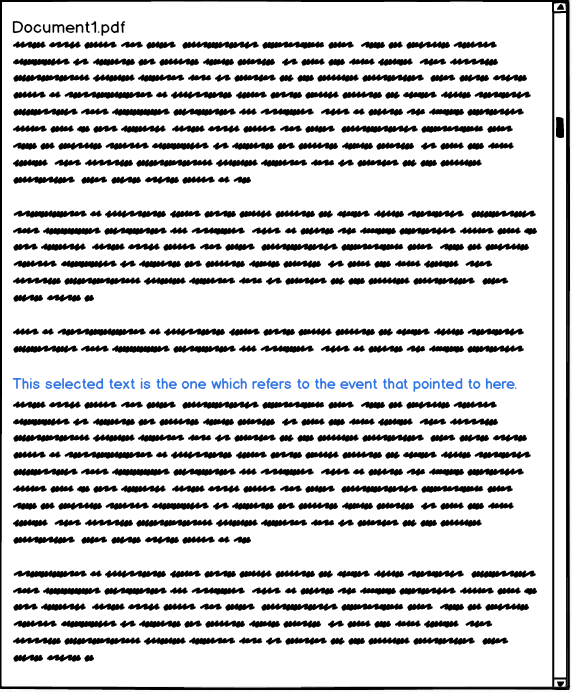
\includegraphics[scale=0.75]{viewDoc.png}
\centering
\end{figure}
\par In the Document Viewer (see Figure \ref{fig:viewDoc}), it should be noted that the relevant sentence that produced the event, which the user interacted with to view this, is highlighted. This allows the user to see in context the event, as they can read the text surrounding this, giving them a better understanding of what occurred. This also allows the user to swap between the system and the documents, viewing how each event has been produced, and judging how effective the system is. In addition, if the user is interested in a certain event, they can jump to the document and just read the part related to that event, instead of having to read the entire document just to obtain more information on one aspect of it. This being extremely beneficial for large documents, as it is both time-efficient, and thereby cost-effective, as the user can focus on that specific aspect of the document (i.e. the text surrounding the sentence that produced the event) instead of having to re-read the chapter, or even the whole document. It should be noted that this tool should not replace the reading of highly sensative law documents, as the user may require the full context of the document, but it can serve as a time-effective tool after the user has done this. Since it allows them to skip through the document event-by-event, and focus on certain events and areas of the document that they may need to revisit.
//wireframes, reason for this, why no color, why no other layout?, update to new system










